%D�finir le format du document: papier, taille de police, type de document, etc.
\documentclass[a4paper, 11pt]{article}

%%%%%%%%% Packages externes utilis�s %%%%%%%%%%%%%%%%%%%
\usepackage[french]{babel}
\usepackage[latin1]{inputenc}
\usepackage[T1]{fontenc}
\usepackage{verbatim}
\usepackage{graphicx}
\usepackage{epstopdf}
\usepackage{amsmath}
\usepackage{amssymb}
\usepackage{macro}
\usepackage{algorithm}
\usepackage{algorithmic}
\usepackage{xcolor}
\usepackage{textcomp}
\usepackage{listings}
\lstset{
language=C,
basicstyle=\normalsize, % ou �a==> basicstyle=\scriptsize,
upquote=true,
aboveskip={1.5\baselineskip},
columns=fullflexible,
showstringspaces=false,
extendedchars=true,
breaklines=true,
showtabs=false,
showspaces=false,
showstringspaces=false,
identifierstyle=\ttfamily,
keywordstyle=\color[rgb]{0,0,1},
commentstyle=\color[rgb]{0.133,0.545,0.133},
stringstyle=\color[rgb]{0.627,0.126,0.941},
}
%\usepackage{algorithm2e}


%La mise en page du rapport, NE PAS MODIFIER.
\usepackage{geometry}
 \geometry{
 a4paper,
 left=20mm,
 right=20mm,
 top=20mm,
 bottom=20mm,
 }

%%%%%%%%% Le corps du document entre begin et end %%%%%%%%%%%%%%%%%%%
\begin{document}

\section*{Video Stream}
\label{sec:Video_Stream}

\noindent Once connected to the GoPro camera, the drone can send a video stream to an other device.


\subsection*{Prerequisites}
\label{sec:Prerequisites}

\paragraph{Request} First of all to request the data stream, you have to connect to the WiFi network of the drone and you need to initialize a TCP connection to the controller in order that it know the host.

\paragraph{WiFi} To connect to the WiFi network, you only have to turn on the drone and the controller, after that connect your device to WiFi named "SoloLink-\_\_\_\_\_\_" and enter the  password "sololink".

\paragraph{TCP} To initialize the TCP connection you have two possibility : simulate it with an utility like netcat or open a socket with an handmade program. In both cases you have to connect to the port 5502 and the address "10.1.1.1" (IP address of the controller)

\begin{lstlisting}
nc 10.1.1.1 5502

or

s = socket(PF_INET, SOCK_STREAM, 0);
serv_addr.sin_family = AF_INET;
serv_addr.sin_addr.s_addr = inet_addr ("10.1.1.1");	// Address of the server
serv_addr.sin_port = htons (5502);	// Port of the server
memset (&serv_addr.sin_zero, 0, sizeof(serv_addr.sin_zero));
connect (s, (struct sockaddr *)&serv_addr, sizeof serv_addr);
\end{lstlisting}


\subsection*{Get video stream}
\label{sec:stream}

\paragraph{} To get the video stream you have several possibilities :

\paragraph{.} You can directly get it with a software like VLC, opening a file named "sololink.sdp" with the following lines :

\begin{lstlisting}
c=IN IP4 10.1.1.1
m=video 5600 RTP/AVP 96
a=rtpmap:96 H264/90000
t=0 0
\end{lstlisting}

\paragraph{.} An other way is to create a UDP server in an handmade program, listening on the port 5600 and interpret the received frames. This method remains the most complicated to set up.

\begin{lstlisting}
s2 = socket (PF_INET, SOCK_DGRAM, 0);
locAddr.sin_family = AF_INET;
locAddr.sin_addr.s_addr = INADDR_ANY;
locAddr.sin_port = htons (5600);	// Listening port
memset (&locAddr.sin_zero, 0, sizeof(locAddr.sin_zero));
bind (s2, (struct sockaddr *)&locAddr, sizeof locAddr);

memset(buf, 0, BUFFER_LENGTH);
recsize = recvfrom(s2, (void *)buf, BUFFER_LENGTH, 0, (struct sockaddr *)&serv_addr, &fromlen);
\end{lstlisting}

\paragraph{.} Third possibility, use the library GStreamer and more specialy in this case his launch command. To install this library refer to the installation manuals in the sources. Thus with the command line below we obtain and display the video stream in the same way than with VLC.

\begin{lstlisting}
gst-launch-1.0 -v udpsrc port=5600 caps = "application/x-rtp, media=(string)video, clock-rate=(int)90000, encoding-name=(string)H264, payload=(int)96" ! rtph264depay ! decodebin ! videoconvert ! autovideosink
\end{lstlisting}

\paragraph{.} Last solution, use the library GStreamer again but in this case in an handmade program. To understand each part of the program, we advise you to refer to the documentation in the sources but the main thing to know is that to get the same result than before we only have to call the function "gst\_parse\_launch" where we put the exactly same command line in parameter. The "gst\_init" function must be call before all and can have "NULL" parameters. "gst\_element\_get\_bus" is use to put the pipeline on the bus, "gst\_element\_set\_state" to start playing the video and the "loop" functions are used to initialize and run the video stream.

\begin{lstlisting}
/* Initialize GStreamer */
gst_init(&argc, &argv);

/* Build the pipeline */
pipeline = gst_parse_launch("-v udpsrc port=5600 caps = \"application/x-rtp, media=(string)video, clock-rate=(int)90000, encoding-name=(string)H264, payload=(int)96\" ! rtph264depay ! decodebin ! videoconvert ! autovideosink", NULL);
bus = gst_element_get_bus(pipeline);
	
/* Start playing */
ret = gst_element_set_state(pipeline, GST_STATE_PLAYING);
	
/* Loop */
loop = g_main_loop_new(NULL, FALSE);
g_main_loop_run(loop);
\end{lstlisting}


\subsection*{Protocol}
\label{sec:Protocol}

\paragraph{} As previously said, the video stream is broadcast using the UDP protocol. In our case, we listen packets from 10.1.1.1 (controller IP address) on the port 5600. The format of a UDP frame is in the following form :

\begin{figure}[H]
	\centering
		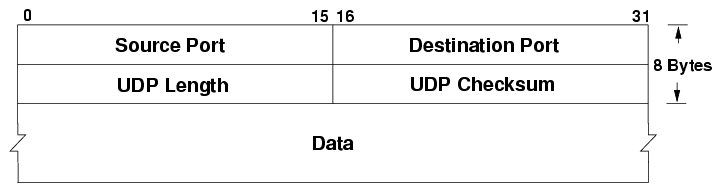
\includegraphics[scale=0.5]{./images/UDP_Construction.png}
		\caption{Construction of an UDP frame}
	\label{fig:UDP_Construction}
\end{figure}

\paragraph{} Encapsulated into this protocol we find the RTP/AVP protocol. This one is done for delivering audio and video. In our case we only deliver video, so we use a payload of type dynamic for only video (H264 AVC) which matches with the MPEG-4 format. More, the clock rate is of 90000 Hz.

\begin{figure}[H]
	\centering
		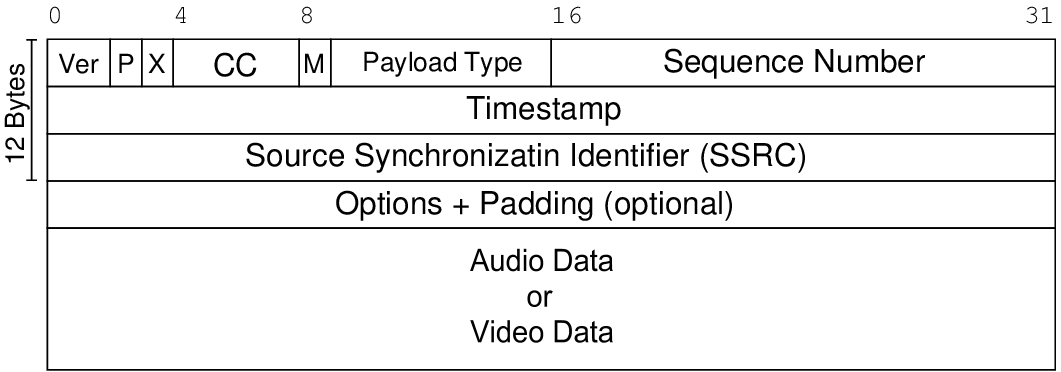
\includegraphics[scale=0.3]{./images/RTP_Construction.png}
		\caption{Construction of an RTP frame}
	\label{fig:RTP_Construction}
\end{figure}





\subsection*{Sources}
\label{sec:Sources}

\begin{itemize}
\item Streaming live video from the 3DR Solo : https://www.markturner.net/2017/02/06/streaming-live-video-from-the-3dr-solo/
\item Install GStreamer on macOS : https://gstreamer.freedesktop.org/documentation/installing/on-mac-osx.html\#InstallingonMacOSX-Build
\item Install GStreamer on linux : https://gstreamer.freedesktop.org/documentation/installing/on-linux.html
\item Install GStreamer on windows : https://gstreamer.freedesktop.org/documentation/installing/on-windows.html
\item GStreamer theory : https://nicolargo.developpez.com/tutoriels/audio/gstreamer-theorie/
\item GStreamer documentation : https://gstreamer.freedesktop.org/documentation/index.html
\item Get video stream with GStreamer in the command line : https://gist.github.com/esrever10/7d39fe2d4163c5b2d7006495c3c911bb
\item Get video stream with GStreamer in a program c : https://stackoverflow.com/questions/41698656/convert-gstreamer-command-to-c-code
\end{itemize}




\end{document}
